\chapter{Qualitätsszenarien}
\label{sec:qualityscenarios}
\section{Qualitätsbaum}

Der Qualitätsbaum und die Qualitätsziele wurden anhand der Anforderungen im Kapitel \ref{requirements} definiert.

\begin{figure}[H]
	\centering
	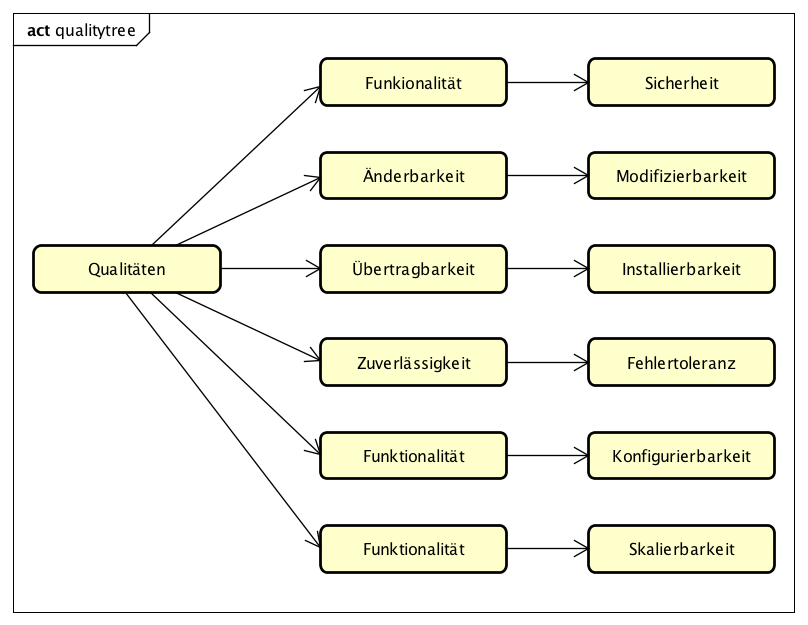
\includegraphics[scale=0.7]{qualitytree.png}
	\caption{Qualitätsbaum}
\end{figure}

\begin{table}[H]
	\centering
	\caption{Qualitätsziele}
	\begin{tabular}{ | p{3cm} | p{3.5cm} | p{6.5cm} | p{1cm} | }
		\toprule
		{\textbf{Merkmal}} & {\textbf{Untermerkmal}} & {\textbf{Szenario}} & {\textbf{Prio}} \\
		\midrule
		Funktionalität & Sicherheit & Q1: Der Zugriff auf sensitive Daten (\textit{\gls{PCI}}) darf nicht möglich sein & 1 \\ \hline
		Änderbarkeit & Modifizierbarkeit & Q2: Anpassungen an der Software sollen einfach eingeführt werden können & 1 \\ \hline
		Übertragbarkeit & Installierbarkeit & Q3: Die Applikation soll ohne Unterbrechung des Dienstes installiert werden können. & 2 \\ \hline
		Zuverlässigkeit & Fehlertoleranz & Q4: Der Händler soll sich, bei korrektem Ausfüllen der Daten, registrieren können & 2 \\ \hline
		Funktionalität & Konfigurierbarkeit & Q5: Konfigurationsänderungen an der Applikation können ohne Unterbruch durchgeführt werden. & 2 \\ \hline
		Funktionalität & Skalierbarkeit & Q6: Die Applikation soll schnell horizontal skaliert werden können. & 2 \\
		\bottomrule
	\end{tabular}
\end{table}
\newpage
\section{Bewertungsszenarien}

Damit die angepasste Architektur bewertet werden kann, wurden folgenden Bewertungsszenarien definiert. 

\subsection{Szenario: Der Zugriff auf sensitive Daten (PCI) darf nicht möglich sein}
%% https://www.pcisecuritystandards.org/document_library
Nach PCI Standard müssen Kartendaten geschützt und unberechtigter Zugriff verhindert werden. Die Applikation selber hält keine Kartendaten sondern hat Schnittstellen zu Systeme welche dies tun. Obschon diese Anwendungen in einer separat geschützten Zone stehen, ist die Firewall für einige Systeme geöffnet, welche es einem Angreifer ermöglichen könnten an Daten zu kommen.

\begin{table}[H]
	\centering
	\begin{tabular}{ | p{3cm} | p{12cm} | }
		\toprule
		Geschäftsziel & Damit SIX Kartendaten verarbeiten kann müssen die \textit{\gls{PCI}} Standards eingehalten werden. Die Händler werden in einem System mit sensitiven Daten aufgesetzt, auf dieses System soll kein Zugriff möglich sein. \\ \hline
		Auslöser & Ein Krimineller versucht an Kartendaten zu gelangen. \\ \hline
		Reaktion & Der Zugriff über die Schnittstelle zum System ist nur schreibend und wird überwacht. Systeme, auf welche lesend zugegriffen wird, haben keinen Zugriff auf \textit{\gls{PCI}} relevante Systeme. Unregelmässigkeiten werden geloggt. \\
		\bottomrule
	\end{tabular}
\end{table}

\subsection{Szenario: Anpassungen an der Software sollen schnell eingeführt werden können}

Es muss möglich sein neue Businessanforderungen und Fehlerbehebungen in der Software schnell nach der Umsetzung in der produktiven Plattform zu integrieren ohne das ein Unterbruch des Dienstes für den Benutzer ersichtlich wird.

\begin{table}[H]
	\centering
	\begin{tabular}{ | p{3cm} | p{12cm} | }
		\toprule
		Geschäftsziel & Die Anforderungen vom Business (z.B. Risk) oder Fehler in der Software muss möglichst zeitnah ausgerollt werden. \\ \hline
		Auslöser & Eine Änderung oder ein Fehler führen zu rechtlich inkonsistentem Zustand. \\ \hline
		Umgebung & Produktion\\ \hline
		Systembestandteil & Ganzes System. \\ \hline
		Reaktion & Die Software wird vom Entwickler behoben und kann nach Abnahme des zuständigen Stakeholders selbstständig in der Produktion ausgerollt werden. \\ \hline
		Zielwerte & Durchlauf von Abnahme bis zur produktiven Benutzbarkeit soll in unter 10 Minuten erreicht werden.\\
		\bottomrule
	\end{tabular}
\end{table}

\subsection{Szenario: Die Applikation soll einfach auf unterschiedlichen Umgebungen installiert werden können}

Die Applikation soll sowohl intern für Tester als auch extern für Businessabnahmen oder zur Skalierung einfach in verschiedenen Umgebungen installiert werden können.

\begin{table}[H]
	\centering
	\begin{tabular}{ | p{3cm} | p{12cm} | }
		\toprule
		Geschäftsziel & Die Applikation ist standortunabhängig in verschiedenen Versionen verfügbar. \\ \hline
		Auslöser & Ein Businessvertreter möchte die Applikation zur Abnahme zur Verfügung gestellt bekommen. \\ \hline
		Reaktion & Die Applikation wird in einer neuen Umgebung dem Businessvertreter zugänglich gemacht. \\ \hline
		Zielwert & Eine neue Umgebung ist in weniger als 10min verfügbar. \\
		\bottomrule
	\end{tabular}
\end{table}

\subsection{Szenario: Der Händler soll sich, bei korrektem Ausfüllen der Daten, registrieren können}

Das Abschicken der Registrierungsdaten soll bei validem Inhalt jederzeit möglich sein auch wenn die Software gerade neu installiert wird oder eine Komponente einen Fehler/Ausfall hatte.

\begin{table}[H]
	\centering
	\begin{tabular}{ | p{3cm} | p{12cm} | }
		\toprule
		Geschäftsziel & Der Händler füllt das Formular korrekt aus und meldet sich damit bei der SIX als Kunde an. \\ \hline
		Auslöser & Der Händler drückt den Registrierungsknopf am Ende des Pagewizards \\  \hline
		Reaktion & Der Händler kriegt eine Bestätigung, dass sein Formular bearbeitet wird. \\ \hline
		Zielwerte & Unabhängig der Verfügbarkeit der Umsysteme muss ein Händler erfolgreich die Registrierung abschliessen können \\
		\bottomrule
	\end{tabular}
\end{table}
\newpage

\subsection{Szenario: Konfigurationsänderungen an der Applikation können ohne Unterbruch durchgeführt werden}

Auf dem produktiven System können Konfigurationsänderungen an der Applikation während des laufenden Betriebs durchgeführt werden ohne das ein Unterbruch des Dienstes nötig wird.

\begin{table}[H]
	\centering
	\begin{tabular}{ | p{3cm} | p{12cm} | }
		\toprule
		Geschäftsziel & Eine Änderung an einer Einstellung muss geändert oder ein Feature aktiviert werden. \\ \hline
		Auslöser & Der Entwickler macht einen Commit in das Konfigurationsrepository\\ \hline
		Reaktion & Die Anwendungen werden via Message Bus benachrichtig und aktualisieren die Einstellungen \\ \hline
		Zielwerte & Die Änderungen werden ohne Neustart der Anwendung übernommen.\\
		\bottomrule
	\end{tabular}
\end{table}


\subsection{Szenario: Die Applikation soll schnell horizontal skaliert werden können.}

Kommt das System durch eine hohe Anzahl sich registrierender Händler unter Last respektive erhören sich die Antwortzeiten, soll es möglich sein die Applikation horizontal zu skalieren um die Antwortzeiten zu senken.

\begin{table}[H]
	\centering
	\begin{tabular}{ | p{3cm} | p{12cm} | }
		\toprule
		Geschäftsziel & Die Antwortzeiten der Applikation bleiben unter einer Sekunde \\ \hline
		Auslöser & Mehrere gleichzeitige Benutzer belasten das System und erhöhen die Antwortzeiten. \\ \hline
		Umgebung & Produktion\\ \hline
		Reaktion & Die Applikation wird horizontal skaliert um die Antwortzeiten zu senken. \\ \hline
		Zielwerte & Skalierung ist voll automatisch oder mit einem Konsolenbefehl möglich. \\
		\bottomrule
	\end{tabular}
\end{table}
